% this file is called up by thesis.tex
% content in this file will be fed into the main document
\chapter{Apendice ejemplos de \LaTeX}
% top level followed by section, subsection

    \section{\textcolor{Azul}{Ejemplo de sección en color azul}}

    \section{Ejemplo de tablas}

        Antes de comenzar, se definen  en la tabla ~\ref{tab:tabla} los parámetros y variables utilizadas

        %%%%%%%%Tabla Nombres de parámetros
        \begin{table}[htdp]                             %Inicia el entorno table debajo del texto
            \centering\                                     %   centra la tabla
                \begin{tabular}{||c | c ||}                     %inicia entorno tabular con doble línea en las orillas, 2 columnas con el contenido centrado (c)
                \hline                                          %inserta línea horizontal
                \hline
                Nombre Parámetro/Variable & Símbolo\\
                \hline
                \hline
                Masa del péndulo & $m$ \\
                \hline
                Masa del carro & $M$\\
                \hline
                Distancia del eje de giro al centro de masa & $l$ \\
                \hline
                Aceleración gravitatoria & $g$ \\
                \hline
                Momento de inercia péndulo respecto del eje de giro& $J$ \\
                \hline
                Ángulo del péndulo respecto del eje vertical & $\theta$\\
                \hline
                Velocidad angular del péndulo & $\dot{\theta}$, $\omega$\\
                \hline
                Distancia del carro respecto al centro del riel & x\\
                \hline
                Velocidad del carro & $\dot{x}$, $v$\\
                \hline
                \hline
                \end{tabular}
            \caption[Parámetros dinámicos del carro-péndulo]{\textbf{Parámetros dinámicos del carro-péndulo} - Estos son los valores de parámetros utilizados en el diseño y las simulaciones, corresponden a los valores reales.}
            \label{tab:tabla}                              %etiqueta para referencia
        \end{table}

    \section{Ejemplo de MATLAB (según Jesús)}

        %inserción de codigo de Matlab
        %Es conveniente sangrarlo (los de proteco dicen "indentarlo") para que no se encime con los números  de las líneas a la izquierda

        \begin{lstlisting}[frame=single]
        
            % Declaracion de las variables simbolicas
            syms u z1 z2 z3 z4 J m M g l 
            % Matrices involucradas
            E = [J+m*l*l m*l*cos(z1);m*l*cos(z1) M+m] 
            F = [m*g*l*sin(z1);u+m*l*(z3*z3)*sin(z1)] 
            % Despeje
            V = E\F
            
        \end{lstlisting}


    \section{Ejemplo de citas}

        Ejemplo de cita 1 \cite{latex}


        Ejemplo de cita 2 \cite{prime-number-theorem}
        
        
        Ejemplo de cita 3 \cite{WinNT}

    \section{Ejemplo de pseudocódigo}

        \begin{algorithm}[H]
            \KwData{this text}
            \KwResult{how to write algorithm with \LaTeX2e }
            initialization\;
            \While{not at end of this document}
            {
                read current\;
                \eIf{understand}
                {
                   go to next section\;
                   current section becomes this one\;
                }
                {
                   go back to the beginning of current section\;
                }
            }
            \caption{How to write algorithms}
        \end{algorithm}

    \section{Ejemplo de figuras}

        La figura ~\ref{fig:planta}    % Hace referencia a la imagen "planta" el número se inserta automáticamente
        ilustra los compenentes de la planta.

        \begin{figure}
          \centering
            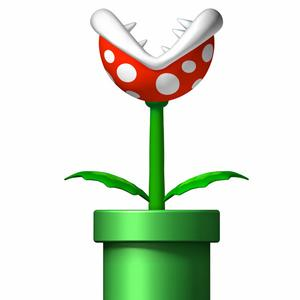
\includegraphics[scale=0.5]{Apendice1/figs/planta.jpg}      % Ruta completa de la imagen, porque se compila desde el archivo tesis.tex
            \caption{Descripción de la planta}            %Pie de imagen
            \label{fig:planta}                            %nombre de referencia
        \end{figure}
        
        \section{Matrices and other arrays in \LaTeX}
            Matrices and other arrays are produced in LaTeX using the \textbf{array} environment. For example, suppose that we wish to typeset the following passage:\\
            The \emph{characteristic polynomial} $\chi(\lambda)$ of the $3 \times 3
            $~matrix
            \[ \left( 
                \begin{array}{ccc}
                    a & b & c \\
                    d & e & f \\
                    g & h & i \end{array} \right)\]


        is given by the formula


            \[ \chi(\lambda) = \left| \begin{array}{ccc}
            \lambda - a & -b & -c \\
            -d & \lambda - e & -f \\
            -g & -h & \lambda - i \end{array} \right|.\] 
            
            
        We can therefore obtain the above formula by typing
        \[ |x| = \left\{ \begin{array}{ll}
                 x & \mbox{if $x \geq 0$};\\
                -x & \mbox{if $x < 0$}.\end{array} \right. \]

% Ejemplo de teoremas

\newtheorem{theorem}{Theorem}[section]
\newtheorem{corollary}{Corollary}[theorem]
\newtheorem{lemma}[theorem]{Lemma}
 

\section{Introduction}
Theorems can easily be defined
 
\begin{theorem}
Let $f$ be a function whose derivative exists in every point, then $f$ is 
a continuous function.
\end{theorem}
 
\begin{theorem}[Pythagorean theorem]
\label{pythagorean}
This is a theorema about right triangles and can be summarised in the next 
equation 
\[ x^2 + y^2 = z^2 \]
\end{theorem}
 
And a consequence of theorem \ref{pythagorean} is the statement in the next 
corollary.
 
\begin{corollary}
There's no right rectangle whose sides measure 3cm, 4cm, and 6cm.
\end{corollary}
 
You can reference theorems such as \ref{pythagorean} when a label is assigned.
 
\begin{lemma}
Given two line segments whose lengths are $a$ and $b$ respectively there is a 
real number $r$ such that $b=ra$.
\end{lemma}

%Agregar en otros archivos.

\chapter{Apendice Matemático}
    \section{Matrices}
    \section{Algebra Lineal}
    \section{Procesos estocasticos}
    \section{Cálculo Vectorial}
    
\chapter{Apendice de Inteligencia Artificial}
    \section{Redes Neuronales}
        \subsection{Perceptron}
        \subsection{Redes neuronales multicapa}
    \section{Agentes}
    \section{Algoritmos geneticos/evolutivos}
        \subsection{NSGA-II}
    \section{Cadenas de Markov}
    \section{Inteligencia de colmena}
    \section{Análisis de sentimiento}
    \section{Rationality}
    
\chapter{Apendice de Game Theory}
    \section{Game Theory} 
    \section{Types of games}
        \subsection{Cooperative or non-cooperative}
        \subsection{Symmetric and asymmetric}
        \subsection{Zero-sum and non-zero-sum}
        \subsection{Simultaneous and sequential}   
        \subsection{Perfect information and imperfect information}
        \subsection{Combinatorial games}
        \subsection{Infinite long games}
        \subsection{Discrete and continuous games}
        \subsection{Differential games}
        \subsection{Many-player and population games}
        \subsection{Stochastic outcomes (and relation to other fields)}
        \subsection{Metagames}
    \section{Collective intentionality}
        
\chapter{Apendice de métodos bayesianos en finanzas}
    \section{Conceptos.(Incluir indice)}